\begin{figure}[H]
\scalebox{0.5}{%
    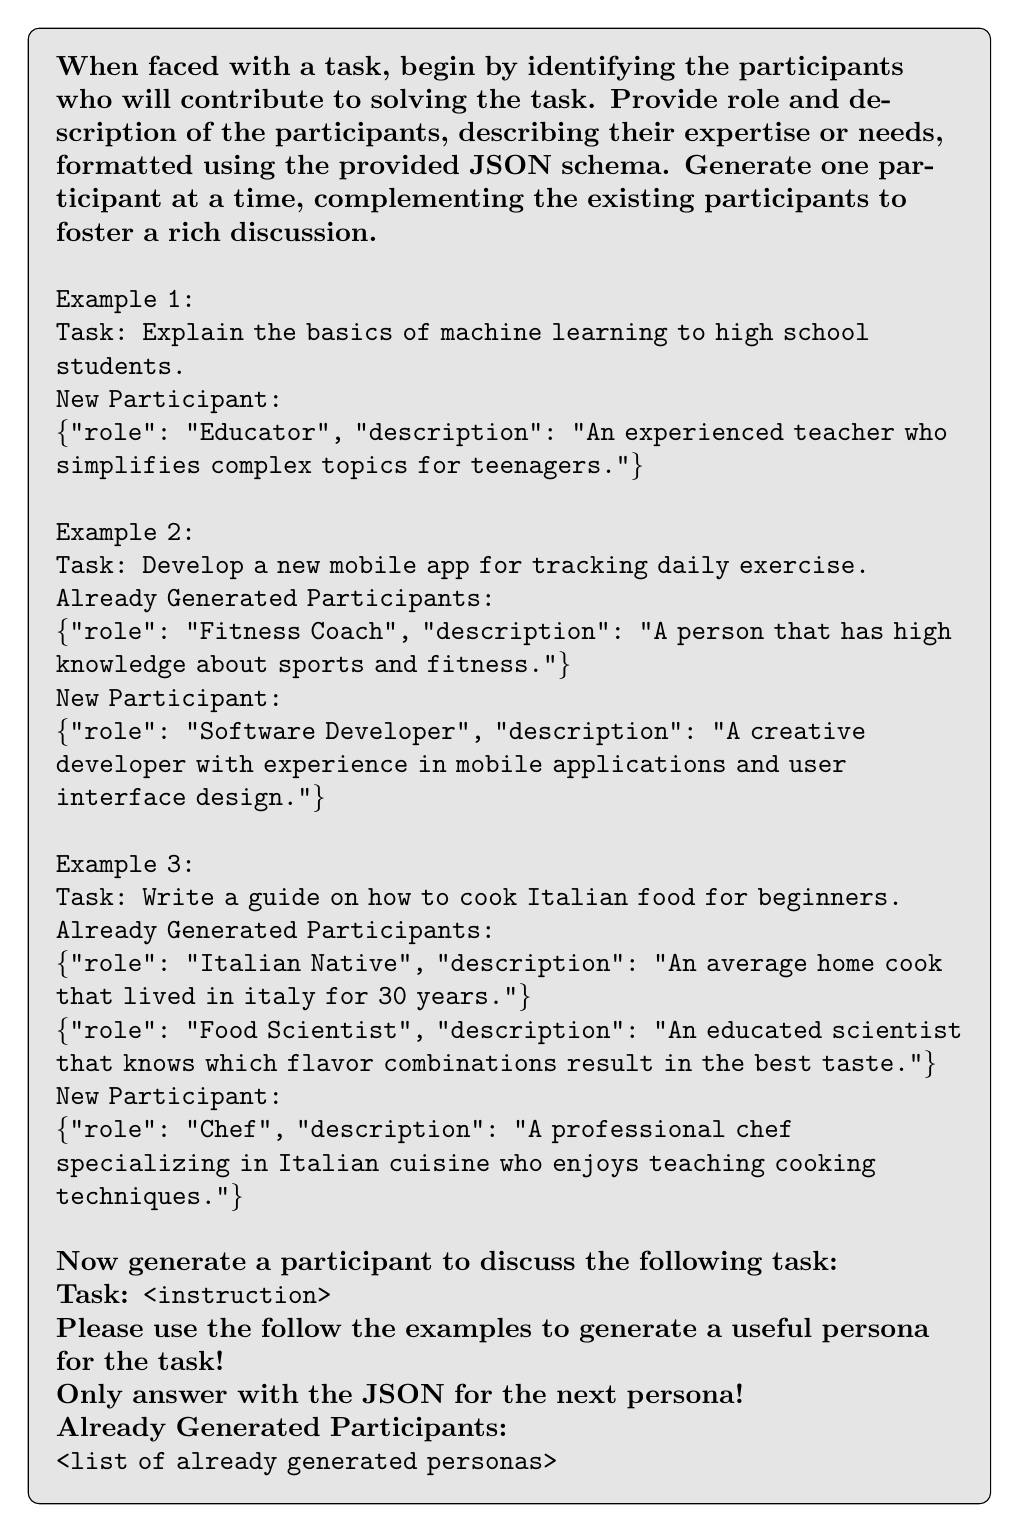
\begin{tikzpicture}
    \node [draw, rectangle, rounded corners, fill=gray!20, text width=0.95\textwidth, inner sep=10pt] (block) {
        \begin{minipage}{\textwidth}
        \textbf{When faced with a task, begin by identifying the participants who will contribute to solving the task. Provide role and description of the participants, describing their expertise or needs, formatted using the provided JSON schema. Generate one participant at a time, complementing the existing participants to foster a rich discussion.}\\
        \\
        \texttt{Example 1:}\\
        \texttt{Task: Explain the basics of machine learning to high school students.}\\
        \texttt{New Participant:}\\
        \texttt{\{"role": "Educator", "description": "An experienced teacher who simplifies complex topics for teenagers."\}}\\
        \\
        \texttt{Example 2:}\\
        \texttt{Task: Develop a new mobile app for tracking daily exercise.}\\
        \texttt{Already Generated Participants:}\\
        \texttt{\{"role": "Fitness Coach", "description": "A person that has high knowledge about sports and fitness."\}}\\
        \texttt{New Participant:}\\
        \texttt{\{"role": "Software Developer", "description": "A creative developer with experience in mobile applications and user interface design."\}}\\
        \\
        \texttt{Example 3:}\\
        \texttt{Task: Write a guide on how to cook Italian food for beginners.}\\
        \texttt{Already Generated Participants:}\\
        \texttt{\{"role": "Italian Native", "description": "An average home cook that lived in italy for 30 years."\}}\\
        \texttt{\{"role": "Food Scientist", "description": "An educated scientist that knows which flavor combinations result in the best taste."\}}\\
        \texttt{New Participant:}\\
        \texttt{\{"role": "Chef", "description": "A professional chef specializing in Italian cuisine who enjoys teaching cooking techniques."\}}\\
        \\
        \textbf{Now generate a participant to discuss the following task:} \\
        \textbf{Task:} \texttt{<instruction>} \\
        \textbf{Please use the follow the examples to generate a useful persona for the task!} \\
        \textbf{Only answer with the JSON for the next persona!} \\
        \textbf{Already Generated Participants:} \\
        \texttt{<list of already generated personas>}
        \end{minipage}
    };
    \end{tikzpicture}
}
\caption{Prompt for the automatic persona assignment. We generate the personas with three iterations of this prompt, adding one persona at a time that complements the ones previously generated.}
\end{figure}
